\documentclass[12pt]{scrartcl}
\usepackage[sexy]{james}
\usepackage[noend]{algpseudocode}
\setlength{\marginparwidth}{2cm}
\usepackage{answers}
\usepackage{array}
\usepackage{tikz}
\usepackage{graphicx}
\newenvironment{allintypewriter}{\ttfamily}{\par}
\usepackage{listings}
\usepackage{xcolor}
\usetikzlibrary{arrows.meta}
\usepackage{color}
\usepackage{mathtools}
\newcommand{\U}{\mathcal{U}}
\newcommand{\E}{\mathbb{E}}
\usetikzlibrary{arrows}
\Newassociation{hint}{hintitem}{all-hints}
\renewcommand{\solutionextension}{out}
\renewenvironment{hintitem}[1]{\item[\bfseries #1.]}{}
\renewcommand{\O}{\mathcal{O}}
\declaretheorem[style=thmbluebox,name={Chinese Remainder Theorem}]{CRT}
\renewcommand{\theCRT}{\Alph{CRT}}
\setlength\parindent{0pt}
\usepackage{sansmath}
\usepackage{pgfplots}

\usetikzlibrary{automata}
\usetikzlibrary{positioning}  %                 ...positioning nodes
\usetikzlibrary{arrows}       %                 ...customizing arrows
\newcommand{\eqdef}{=\vcentcolon}
\newcommand{\tr}{{\rm tr\ }}
\newcommand{\im}{{\rm Im\ }}
\newcommand{\spann}{{\rm span\ }}
\newcommand{\Col}{{\rm Col\ }}
\newcommand{\Row}{{\rm Row\ }}
\newcommand{\dint}{\displaystyle\int}
\newcommand{\dt}{\ {\rm d }t}
\newcommand{\PP}{\mathbb{P}}
\newcommand{\horizontal}{\par\noindent\rule{\textwidth}{0.4pt}}
\usepackage[top=3cm,left=3cm,right=3cm,bottom=3cm]{geometry}
\newcommand{\mref}[3][red]{\hypersetup{linkcolor=#1}\cref{#2}{#3}\hypersetup{linkcolor=blue}}%<<<changed

\tikzset{node distance=4.5cm, % Minimum distance between two nodes. Change if necessary.
         every state/.style={ % Sets the properties for each state
           semithick,
           fill=cyan!40},
         initial text={},     % No label on start arrow
         double distance=4pt, % Adjust appearance of accept states
         every edge/.style={  % Sets the properties for each transition
         draw,
           ->,>=stealth',     % Makes edges directed with bold arrowheads
           auto,
           semithick}}


% Start of document.
\newcommand{\sep}{\hspace*{.5em}}

\pgfplotsset{compat=1.18}
\begin{document}
\title{MATH410: Homework 5}
\author{James Zhang\thanks{Email: \mailto{jzhang72@terpmail.umd.edu}}}
\date{\today}

\definecolor{dkgreen}{rgb}{0,0.6,0}
\definecolor{gray}{rgb}{0.5,0.5,0.5}
\definecolor{mauve}{rgb}{0.58,0,0.82}

\lstset{frame=tb,
  language=Java,
  aboveskip=3mm,
  belowskip=3mm,
  showstringspaces=false,
  columns=flexible,
  basicstyle={\small\ttfamily},
  numbers=left,
  numberstyle=\tiny\color{gray},
  keywordstyle=\color{blue},
  commentstyle=\color{dkgreen},
  stringstyle=\color{mauve},
  breaklines=true,
  breakatwhitespace=true,
  tabsize=3
}

\maketitle

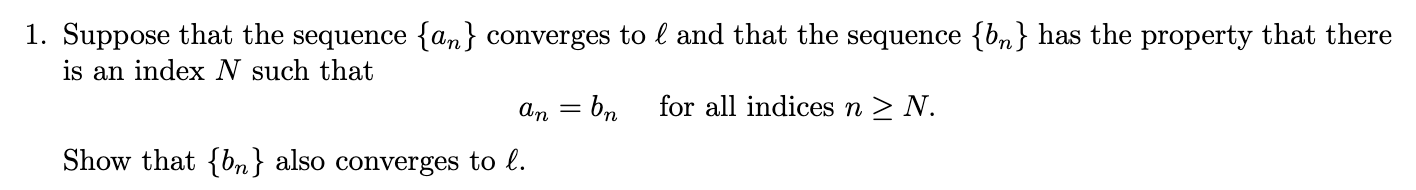
\includegraphics[width=15cm]{1.png}

\begin{proof}
  
  \hfill

  \begin{enumerate}[a.]
    \item False. WLOG, suppose $f$ is monotone increasing. Then it follows that $f(u) \leq f(v) \ \forall \ u, v \in \RR, u < v$. 
    Consider the function $f(x) = 1 \ \forall \ x \in \RR$. Note that this function is monotone increasing. 
    Assume on the contrary now that $f$ is also one-to-one. Note that $f(1) = f(2)$. By definition of one-to-one 
    $1 = 2$ but this is obviously a contradiction, so $f: \RR \to \RR$ is not one-to-one.
    \item True. Assume on the contrary that $f: \RR \to \RR$ is not one-to-one. By definition of strictly increasing, 
    $f(u) < f(v) \ \forall \ u, v \in \RR, u < v$. 
    Since $f$ is not one-to-one, there exists $x_1, x_2 \in \RR$ such that $f(x_1) = f(x_2)$. Choose 
    these points. Let $x_1 < x_2$ WLOG. However, by definition of strictly increasing, $f(x_1) < f(x_2)$
    which is a contradiction, so $f$ is one-to-one.
    \item False. Consider the piecewise function
    \[f(x) = \begin{cases}
      x, x \geq 0\\
      x - 1, x < 0
    \end{cases}\]
    Let us show that $f$ is strictly increasing by considering $x_1, x_2 \in \RR$ and then considering cases. 
    WLOG, let $x_1 < x_2$. For each case, we WTS that $x_1 < x_2 \implies f(x_1) < x_2$. 
    \begin{enumerate}[a.]
      \item $0 \leq x_1 < x_2 \implies x_1 < x_2$ which is true.
      \item $x_1 < 0 \leq x_2 \implies x_1 - 1 < x_2$ which is true.
      \item $0 < x_1 < x_2 \implies x_1 - 1 < x_2 - 1 \implies x_1 < x_2$ which is true. 
    \end{enumerate}
    Therefore, $f$ is strictly increasing. Now we will show that $f$ is not continuous. Let us define 
    two sequences $\{u_n\} = \{\frac{1}{n}\}$ and $\{v_n\} = \{-\frac{1}{n}\}$ whose limits are both
    $0$. Note that $\{f(u_n)\}_{n=1}^\infty = 0 \neq \{f(v_n)\}_{n=1}\infty = -1$. Therefore, 
    for all sequences that converge to $x_0 = 0$, not all image sequences converge to the functional value 
    $f(x_0) = 0$, so $f$ is not continuous.
    \item False. Consider the function 
    \[f(x) = \begin{cases}
      x, x \in \QQ \\ 
      -x, x \notin \QQ
    \end{cases}\]
    Let us prove that this function is one-to-one. Assume on the contrary that $f$ is not one-to-one. 
    Since $f$ is not one-to-one, there exists $x_1 \neq x_2$ such that $f(x_1) = f(x_2)$.
    However, $f(x_1) = f(x_2) \in \QQ \implies x_1 = x_2$ and similarly for $\QQ^c$. Thus, $f$ is 
    one-to-one. Now we will show that $f$ is not monotone. Consider $x_1 = 0, x_2 = \pi$.
    $0 < \pi \implies f(0) < f(\pi) \implies 0 < -\pi$ which is a contradiction.
  \end{enumerate}
\end{proof}

\newpage

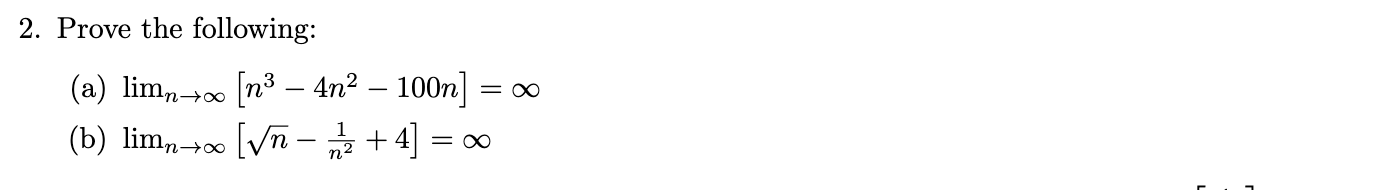
\includegraphics[width=15cm]{2.png}

\begin{proof}
  Let $f$ be odd and suppose that $f: [0, \infty)$ is strictly increasing. We WTS 
  that $f: \RR \to \RR$ is strictly increasing, or that for all $x_1, x_2 \in \RR, x_1 < x_2$ then $f(x_1) < f(x_2)$.
  Consider $x_1, x_2 \in \RR$ such that $0 \leq x_1 < x_2$. Then by definition of strictly increasing, 
  $f(x_1) < f(x_2) \implies -f(x_1) > -f(x_2)$ by multiplying the inequality 
  by $-1$. By definition of odd, $f(-x_1) = -f(x_1)$ and 
  $f(-x_2) = -f(x_2)$. Therefore, by substitution, $f(-x_1) > f(-x_2)$ where $x_1 < x_2 \implies -x_1 > -x_2$. Note that 
  $x_1, x_2 \in [0, \infty) \implies -x_1, -x_2 \in (-\infty, 0]$ and that $(-\infty, 0] \cap [0, \infty) = \RR$. 
  Thus, we have shown that $f: \RR \to \RR$ is strictly increasing.
\end{proof}

\newpage

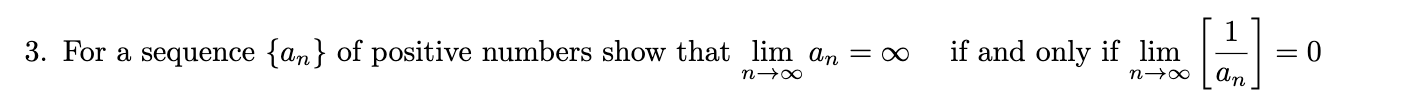
\includegraphics[width=15cm]{3.png}

\begin{proof}
  
  \hfill

  \begin{enumerate}[a.]
    \item Note that polynomials are continuous, and so the quotient is continuous. Let $\{x_n\} \to 1$
    with $x_n \neq 1$. Then 
    \[\dfrac{x_n^4 - 1}{x_n - 1} = \dfrac{(x_n^2 + 1)(x_n + 1) (x_n - 1)}{(x_n - 1)} = (x_n^2 + 1)(x_n + 1)\]
    \[\lim_{x\to 1} \dfrac{x^4 - 1}{x - 1} = \lim_{n\to\infty}(x_n^2 + 1)(x_n + 1) = 4\]
    
    \item $\sqrt{x}$ is continuous because it is the inverse of a strictly increasing funciton, and the denominator 
    is continuous because it is linear, and so the quotient is continuous. Let $\{x_n\} \to 1$, but $x_n \neq 1$. 
    Then 
    \[\dfrac{\sqrt{x_n} - 1}{x - 1} = \dfrac{\sqrt{x_n} - 1}{(\sqrt{x_n} + 1)(\sqrt{x_n} - 1)} = \dfrac{1}{\sqrt{x_n + 1}}\]
    \[\lim_{x \to 1}\dfrac{\sqrt{x} - 1}{x - 1} = \lim_{n\to\infty} \dfrac{\sqrt{x_n} - 1}{x - 1} = \lim_{n\to\infty} \frac{1}{\sqrt{x_n + 1}} = \frac{1}{2}\]
  \end{enumerate}

\end{proof}

\newpage 

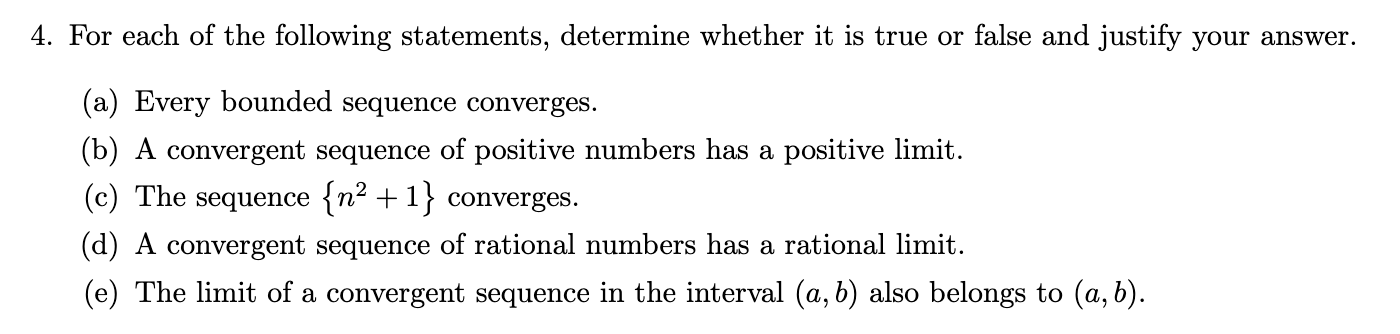
\includegraphics[width=15cm]{4.png}

\begin{proof}

\hfill

\begin{enumerate}[a.]
  \item Note that 
  \[\frac{1 + \frac{1}{x}}{1 + \frac{1}{x^2}} = (1 + \frac{1}{x})(\frac{1}{1 + \frac{1}{x^2}}) = (\frac{x + 1}{x})(\frac{x^2}{x^2 + 1}) = \frac{x(x+1)}{x^2 + 1}\]
  Let $\{x_n\} \to 0$ but $x_n \neq 0$. Then 
  \[\lim_{x\to 0} \frac{1 + 1/x}{1 + 1/x^2} = \lim_{n\to\infty} \frac{x_n(x_n + 1)}{(x_n^2 + 1)} = \frac{0(1)}{1} = 0\]
  \item Note similar to above that 
  \[\frac{1 + 1/x^2}{1 + 1/x} = (1 + 1/x^2)(\frac{1}{1 + 1/x}) = (\frac{x^2 + 1}{x^2})(\frac{x}{x + 1}) = \frac{x^2 + 1}{x(x+1)}\] 
  \[= \frac{1}{x^2 + x} + \frac{x^2}{x^2 + x} = \frac{1}{x^2 + x} + \frac{x}{x + 1}\]
  Let $\{x_n\} \to 0$ but $x_n \neq 0$. Then 
  \[\lim_{x \to 0} \frac{1 + 1/x^2}{1 + 1/x} = \lim_{n\to\infty} \frac{1}{x^2 + 1} + \lim_{n\to\infty} \frac{x}{x+1} = \infty + 1 = \infty\]
  We can break up the above into two limits by limit rules.
  \item Note that 
  \[\frac{1 + 1/(x-1)}{2 + 1/(x-1)^2} = \frac{x}{x-1} * \frac{(x-1)^2}{2(x-1)^2 + 1} = \frac{x(x-1)}{2(x-1)^2 + 1}\]
  Let $\{x_n\} \to 1$ but $x_n \neq 1$. Then 
  \[\lim_{x\to 1} \frac{1 + 1/(x-1)}{2 + 1/(x-1)^2} = \lim_{n\to\infty} \frac{x_n(x_n - 1)}{2(x_n-1)^2 + 1} = \frac{0}{1} = 0\]

\end{enumerate}

\end{proof}

\newpage 

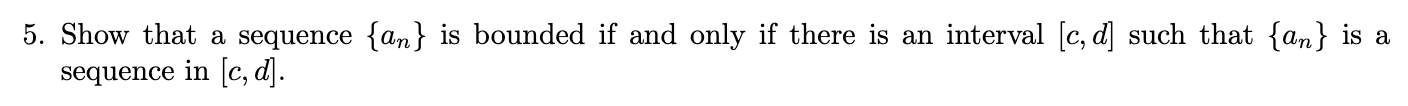
\includegraphics[width=15cm]{5.png}

\begin{proof}

\hfill

\begin{enumerate}[i.]
  \item First let us show that $\underset{x\to 0}{\lim}f(x) = 0$. Let $\{x_n\} \to 0$ but $x_n \neq 0$.
  Observe that $|f(x_n)| = |f(x_n) - 0| \leq M|x_n|^2 = M|x_n^2| = M|x_n^2 - 0|$. Since $\{x_n\} \to 0$ then 
  $\{x_n^2\} \to 0$ by the product property. Since $M > 0$, by the Comparison Lemma, 
  then $\{f(x_n)\} \to 0 \implies \underset{n\to\infty}{\lim}f(x_n) = 0 \implies \underset{x\to 0}{\lim}f(x) = 0$.
  \item Now for $\underset{x\to 0}{\lim}\frac{f(x)}{x}$, let $\{x_n\}\to 0$ but $x_n \neq 0 \ \forall \ n \in \NN$. 
  Observe that 
  \[|f(x_n)| \leq M|x_n|^2 \implies |\frac{f(x_n)}{x_n} - 0| \leq M|x_n - 0|\]
  by dviding both sides by $|x_n|$, and so by the Comparison Lemma once more, 
  \[\{\frac{f(x_n)}{x_n}\} \to 0 \implies \lim_{n\to\infty}\frac{f(x_n)}{x_n} = 0 \implies \lim_{x\to 0}\frac{f(x)}{x} =0\]
\end{enumerate}

\end{proof}

\newpage 

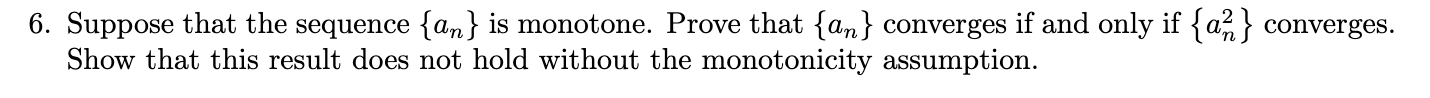
\includegraphics[width=15cm]{6.png}

\begin{proof}
  First let us show that this function is continuous at $0$. We will use the $\epsilon-\delta$ criterion. 
  By a theorem, given $f: D \to \RR, x_0 \in D$, if $f$ satisfies the $\epsilon-\delta$ criterion at 
  $x=0$, then $f$ is continuous at $x=0$. Thus, let $\epsilon > 0$ be given and let $\delta = \frac{\epsilon}{\max(|m_1|, |m_2|)}$. 
  Note that $\delta > 0$. If 
  $|x - 0| < \delta$ then 
  \[|f(x) - f(0)| = |m_*x + 4 - 4| = |m_* x| = |m_*||x-0| < |m_*|\delta = \] 
  \[|m_*|\frac{\epsilon}{\max(|m_1|, |m_2|)}< \epsilon\]
  where $m_* = \begin{cases}
    m_1, x \leq 0\\
    m_2, x \geq 0
  \end{cases}$ and the last step because $\frac{|m_*|}{\max(|m_1|, |m_2|)} \leq 1$ always. Therefore, $f$ is continuous at $x = 0$. Now let us show that $f$ is not 
  differentiable. Consider $\{x_n\} \to 0$ but $x_n \neq 0 \ \forall \ n$. 
  \[\lim_{x\to 0}\frac{f(x) - f(0)}{x - 0} = \begin{cases}
    \underset{n\to\infty}{\lim} \frac{m_1 x_n + 4 - 4}{x_n} = m_1, x \geq 0\\
    \underset{n\to\infty}{\lim} \frac{m_2x_n + 4 - 4}{x_n} = m_2, x < 0
  \end{cases}\]
  Since $m_1 \neq m_2$, this limit is not defined, and so $f$ is not differentiable.
\end{proof}

\newpage 

\includegraphics[width=15cm]{7.png}

\begin{proof}
  
\hfill

For all of these problems, let $\{x_n\} \to 1$ but $x_n \neq 1 \ \forall \ n \in \NN$. 
We seek to find
\[\lim_{x\to 1} \frac{f(x) - f(1)}{x-1}\]

\begin{enumerate}[a.]
  \item Consider 
  \[\lim_{x\to 1}\frac{f(x) - f(1)}{x-1} = \lim_{x\to 1} \frac{\sqrt{x + 1} - \sqrt{2}}{x - 1} = \lim_{x\to 1} \frac{x + 1 - 2}{(x-1)(\sqrt{x+1} + \sqrt{2})}\]
  by multiplying by the conjugate.
  \[ = \lim_{x\to 1} \frac{1}{\sqrt{x + 1} + \sqrt{2}} = \lim_{n\to\infty} \frac{1}{\sqrt{x_n + 1} + \sqrt{2}} = \frac{1}{2\sqrt{2}}\]
  \item Next 
  \[\lim_{x\to 1}\frac{f(x) - f(1)}{x - 1} = \lim_{x \to 1} \frac{x^3 + 2x - 3}{x - 1} = \lim_{n\to\infty} \frac{(x_n^2 + x_n + 3)(x_n - 1)}{x_n - 1}\]
  \[ = \lim_{n\to\infty}(x^2_n + x_n + 3) = 5\]
  \item Finally 
  \[\lim_{x\to 1}\frac{f(x) - f(1)}{x-1} = \lim_{x\to 1} \frac{\frac{1}{1+x^2} - \frac{1}{2}}{x-1} = \lim_{x\to 1} \frac{\frac{2 - 1 - x^2}{1 + x^2}}{x-1} = \lim_{x\to 1}\frac{1-x^2}{(x-1)(1+x^2)}\]
  \[\lim_{x\to 1} \frac{(1+x)(1-x)}{(x-1)(1+x^2)} = \lim_{n\to\infty}-1 * \frac{1 + x_n}{1 + x_n^2} = -1\]
\end{enumerate}
\end{proof}

\newpage 

\includegraphics[width=15cm]{8.png}

\begin{proof}
  
\hfill

Since $f$ is differentiable, we know that the limit 
\[\lim_{x\to x_0} \frac{f(x) - f(x_0)}{x - x_0}\]
exists for all $x_0 \in \RR$. By the definition of bounded, $\exists M > 0$ such that 
$|x_n| \leq M \ \forall \ n \in \NN$. Furthermore, $f(x_n) = 0 \ \forall \ n$ except for 
when $n = m$. Consider the interval $I = [a, b], a, b \in \RR$ such that $m \notin I$. By the Sequential Compactness Theorem, there exist a subsequence $\{x_{n_k}\}$  that converge to a point in the interval, say $x_0$, but 
modify the subsequence such that it never equals $0$ for all $k$. 
Since $x_0 \neq m \implies f(x_0) = 0$ as desired. 
Now let us show that the derivative $f'(x_0) = 0$.
\[\lim_{x\to x_0}\frac{f(x) - f(x_0)}{x - x_0} = \lim_{n\to\infty}\frac{f(x_{n_k}) - f(x_0)}{x_{n_k} - x_0} = \lim_{n\to\infty}\frac{f(x_{n_k}) - 0}{x_{n_k} - x_0}\]
\[\lim_{n\to\infty} \frac{0}{(x_{n_k} - x_0)} = 0 = \lim_{x\to x_0} \frac{f(x) - f(x_0)}{x - x_0} = f'(x_0)\]
Note that the numerator is, by construction, always precisely equal to $0$ since $f(x_{n_k}) = 0 \ \forall \ k$, 
whereas the denominator approaches $0$ but will never actually be $0$.

\end{proof}

\end{document}

